\chapter{Esperiments}

\label{ch:experiments}

In this Chapter, we'll use the \texttt{atarieyes} software to test the
effectiveness of the ideas presented in this thesis. The purpose of these
experiments is both to demonstrate that a features extractor can be learnt
with the method proposed, and to show how these features can be used
in combination with the Restraining Bolt for complex RL tasks.

We'll look at two environments: Breakout and Montezuma's Revenge. For the
first we'll test the training process of the features extractor, while the
second is used for a more complete demonstration about the possibilities (we
proceed from learnt features to the application of the Restraining Bolt).

% Page too short: don't break here
\let\sectionbreak\dontbreakhere

\section{Breakout}

\label{sec:exp-breakout}

The first environment we'll see is the famous Atari game ``Breakout''.
A frame of this game is shown in Figure~\ref{fig:breakout-frame}.
\begin{figure}
	\centering
	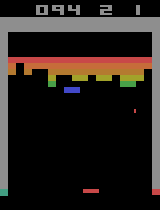
\includegraphics[height=3cm]{./imgs/br1.png}
	\caption{A frame from the Atari game ``Breakout''.}
	\label{fig:breakout-frame}
\end{figure}
The goal is to hit all the bricks with the ball (the small orange dot). Every
time one brick is eliminated, the environment produces a positive reward. The
agent, through the four actions available, \const{NoOp}, \const{Fire},
\const{Right} and \const{Left}, can move the paddle at the bottom and direct
the ball. Every time the paddle misses the ball, the agent loses a life.
However, during training, we terminate and reset the episode at this event.

The exact environment name for this game is \verb|BreakoutDeterministic-v4|.


\subsection{Definitions}

We now define two propositional symbols, \const{Full} and \const{Empty}, and
we apply the proposed model and training procedure to learn their Boolean
valuation function. The intended interpretation of these two proposition
is:
\begin{description}
	\item [\const{Full}] should be true when the area is full of bricks.
	\item [\const{Empty}] should be true when there are no bricks inside the
		area.
\end{description}
The area which we're talking about is shown in
Figure~\ref{fig:breakout-fluents}. The orange rectangle which contains the
intended set of bricks is also the fluents region. So, we've defined two
symbols in one region of the image.
\begin{figure}
	\centering
	\begin{tikzpicture}
		\node [image, tight] (env-br)
			{
\includegraphics[height=4cm]{./imgs/br2.png}};
		\begin{scope}[shift=(env-br.north west), x={(env-br.north east)},
			y={(env-br.south west)}]
			\draw [region box] \boxblueright node (blueright-coord) {};
		\end{scope}
		\matrix (br-fluents) [right=of env-br,
				matrix of nodes, nodes={anchor=west}] {
			\texttt{full}: true when shot 0 of 18 bricks down \\
			\texttt{empty}: true when shot 18 of 18 bricks down \\
		};
		\draw [->, gray] (br-fluents-1-1.west) to (blueright-coord);
		\draw [->, gray] (br-fluents-2-1.west) to (blueright-coord);
	\end{tikzpicture}
	\caption{In this environment we define two fluents and one region.}
	\label{fig:breakout-fluents}
\end{figure}

How could we \emph{describe the behaviour} of these two propositions with
temporal logic? When an episode starts, we know that \const{Full} should be
true, because all bricks are present, initially. This initial condition is
really helpful. Then, \const{Full} and \const{Empty} represent concepts that
are always mutually exclusive. Finally, since the bricks cannot reappear, we
know that the path is forced: the propositions can't return to a previous
configuration. All these descriptions translate to the following \ldl{}
temporal constraint:
\begin{equation}
	\begin{array}{ll}
		\const{Full}\, \land &
		\to \text{initial condition}\\
		\lbox{\true^*} (\lnot \const{Full} \lor \lnot \const{Empty})\, \land &
		\to \text{exclusive propositions}\\
		\lnot \ldiamond{\true^*; \lnot \const{Full}; \true^*}
		(\const{Full} \land \lnot \lend)\, \land &
		\to \text{can't reappear}\\
		\lnot \ldiamond{\true^*; \const{Empty}; \true^*}
		(\lnot \const{Empty} \land \lnot \lend)\, \land \\
		\lnot \ldiamond{\true^*; \const{Full}} \const{Empty} &
		\to \text{not immediately}\\
	\end{array}
	\label{eq:breakout-constraint}
\end{equation}
The conjunction $\land \lnot \lend$ means that we're not referring to the end
of the trace. This is only required in this \ldl{} semantics for finite
traces.

The DFA associated to this temporal constraint is shown in
Figure~\ref{fig:breakout-constraint}. This is the automaton that the software
will use to search among the candidate functions.
\begin{figure}
	\centering
	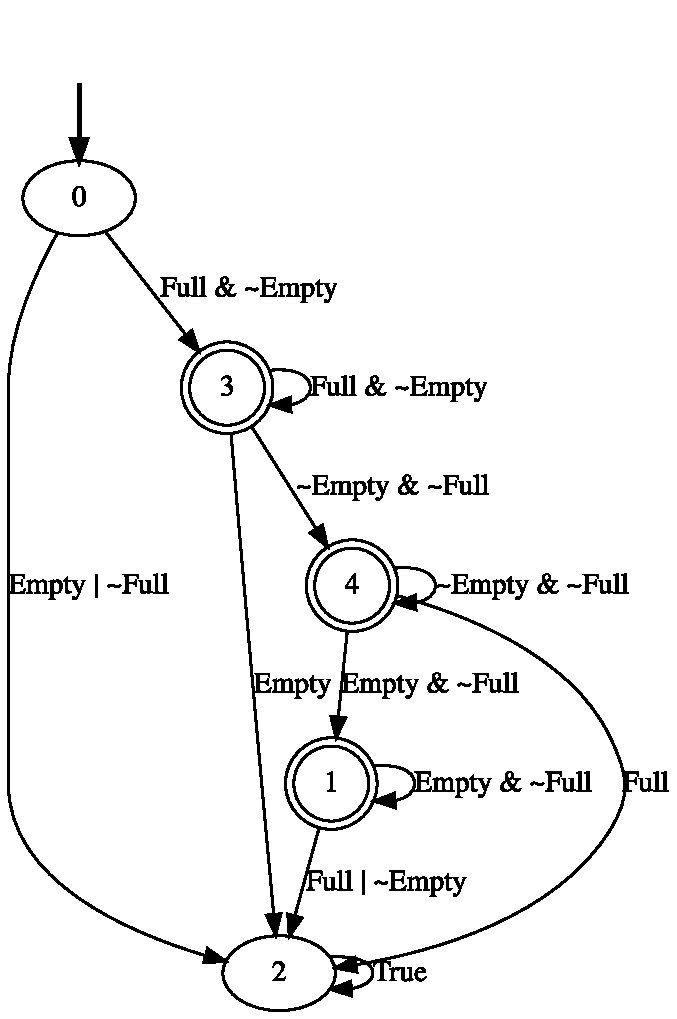
\includegraphics[height=0.5\textheight]{./imgs/br_constraints.pdf}
	\caption{The DFA associated to Equation~\eqref{eq:breakout-constraint}.}
	\label{fig:breakout-constraint}
\end{figure}
As we can see from its structure, the fluents dynamics is relatively simple.
We could have also used the following equivalent formula:
\begin{equation}
	\begin{aligned}
		&\ldiamond{(\const{Full} \land \lnot \const{Empty})^+}
			(\const{End} \,\lor \\
		&\qquad\ldiamond{(\lnot \const{Full} \land \lnot \const{Empty})^+}
			(\const{End} \,\lor \\
		&\qquad\qquad \ldiamond{(\lnot \const{Full} \land \const{Empty})^+}
			\const{End}))
	\end{aligned}
\end{equation}
where the operator $\resym^+$ is an abbreviation of the regular expression
$(\resym; \resym^*)$.
% TODO: draw with tikz

Most states in this automaton are final. In fact, nothing guarantees that the
agent will be able to hit the bricks in every episode. The fluents might not
evolve at all when the agent loses a play.

To specify all these definitions to our software we run:
\begin{minted}{text}
atarieyes features select -e BreakoutDeterministic-v4
\end{minted}
and we select the region of Figure~\ref{fig:breakout-fluents}. Then we
complete the generated file with the fluents names and any of the two temporal
constraints above. The resulting file is shown in
Listing~\ref{lst:breakout-definitions}. 
\begin{listing}
\begin{minted}{json}
{
  "_frame": [
    8, 32, 152, 197
  ],
	"regions": {
		"blue_right": {
			"abbrev": "br",
			"fluents": [
				"br_full",
				"br_empty"
			],
			"region": [
				32, 87, 152, 93
			]
		}
	},
	"constraints": [
		"br_full",
		"[true*](!br_full | !br_empty)",
		"!<true*; !br_full; true*>(br_full & !end)",
		"!<true*; br_empty; true*>(!br_empty & !end)",
		"!<true*; br_full>br_empty"
	]
}
\end{minted}
\caption{The content of \texttt{definitions/BreakoutDeterministic-v4.json}.}
\label{lst:breakout-definitions}
\end{listing}
"\texttt{br}" is just an abbreviation for that region name. Other than that,
the file exactly represents what we've defined so far.


\subsection{Training}

The first step is to train a RL agent on the environment as it is.
Some of the options we've used for the \verb|agent train| command are: a batch
size of 32, learning rate of $0,0001$, double Q-Network update every 10000
steps. To follow the training progress, we run TensorBoard on the agent's log
directory.  The results obtained are shown in
Figure~\ref{fig:breakout-agent-train}.
\begin{figure}
	\centering
	\begin{tikzpicture}
		\begin{axis}[
				metrics, xlabel={episode}, ylabel={cumulative reward},
				width=0.7\textwidth, height=0.25\textheight, ymax=90]
			\addplot table
			{./data/run-agent-episode_metrics_episode_reward.txt};
		\end{axis}
	\end{tikzpicture}
	\caption{Training the RL agent. Plot of the cumulative reward in each
	episode.}
	\label{fig:breakout-agent-train}
\end{figure}

This plot is the cumulative reward achieved in each episode. At the end of the
training, the agent achieves a reward above 70, which means that is able to
hit 70 bricks without ever losing the ball. This was an expected result,
because at this stage, we just want to replicate the results of previous
studies.  The neural network needs time to adapt to the new observations
reached (a frame without bricks is really different for the Q-Network).
However, we stop this training at 4100 episodes, as this is not the main
purpose of this experiment. These performances are, in fact, sufficient to
reach states in which \const{Empty} becomes true. So, we're ready to train the
features extractor.

The fluents are trained from a dataset generated online by a running agent.
So, we start the trained agent from the previous step:
\begin{minted}[escapeinside=“”]{text}
atarieyes agent play “\normalfont<args-file>” -c “\normalfont<checkpoint>” --rand-test 0.1
\end{minted}
where <checkpoint> is any saved agent from the previous training. When
training the feature extractor, the agent should avoid repetitive behaviours,
but try to thoroughly explore the environment. This command selects a
0.1-greedy policy, but we've also experimented with many others, such as
\verb|--rand-eps|. We let this command run and focus on the receiving side.

The network that we use for the encoder is a DBN of size $(N, 50, 20)$. $N$ is
the number of input pixels in our region, but this is computed by the
software and we don't need to specify it. This network contains two RBMs and
generates an encoding of 20 binary units. At first sight, this encoding could
seem quite large. However, we must consider that there are 18 bricks in the
selected region. If we want to learn a representation for these bricks, there
must be at least 18 units. 20 constitutes a nearly-optimal size for this
encoding (we use 20, because the optimal might not be reachable during
training). Also, we've observed that the shallow network $(N, 20)$ is not able
to achieve the same performances as the deep architecture selected here.

First we train the layer number~0, that of size $(N, 50)$, with the following
command:
\begin{minted}{bash}
atarieyes features train --network 50 20 --train blue_right 0
\end{minted}
Other omitted arguments are: the environment, learning rate of $0.001$,
batch size of 50 and regularization factors.

The output of this training is shown by the plots on the left in
Figure~\ref{fig:plot-br-encoder}. The most important is the free energy, shown
in the top left plot, that we've defined in Equation~\eqref{eq:free-energy} at
page~\pageref{eq:free-energy}. A low free energy means that the model is
recognizing the training dataset, because a low energy is associated to a high
probability for the input batches. The second metric, the reconstruction
error, shows the $L_1$ distance between the input images and the reconstructed
images (reconstructions are the most probable images under the encoding
assigned for the true inputs). Minimizing the reconstruction error is not the
training objective of Persistent CD, but it's useful because, unlike the free
energy, we know its scale and lower bound.

\begin{figure}[p]
	\hspace*{-2cm}%
	\begin{minipage}{\textwidth+3.5cm}
	\begin{tikzpicture}
		\pgfplotsset{
			every axis/.append style={
				metrics, width=0.4\textwidth, height=0.25\textheight,
				enlarge x limits=false,
			}
		}
		\begin{axis} [
				name=free energy 0, xlabel={step}, ylabel={free energy}]
			\addplot table
			{./data/run-features-logs0-metrics_free_energy.txt};
		\end{axis}
		\begin{axis}[
				at=(free energy 0.below south), anchor=above north,
				xlabel={step}, ylabel={reconstruction error}, ymin=0, ymax=0.5]
			\addplot table
			{./data/run-features-logs0-metrics_reconstruction_error.txt};
		\end{axis}
		\begin{axis} [
				name=free energy 1,
				at=(free energy 0.right of east), anchor=left of west,
				xlabel={step}]
			\addplot table
			{./data/run-features-logs2-metrics_free_energy.txt};
		\end{axis}
		\begin{axis}[
				at=(free energy 1.below south), anchor=above north,
				xlabel={step}, ymin=0, ymax=0.5]
			\addplot table
			{./data/run-features-logs2-metrics_reconstruction_error.txt};
		\end{axis}
		% Titles
		\node [above, yshift=3ex] at (free energy 0.above north)
			{Training layer 0 -- $(N, 50)$};
		\node [above, yshift=3ex] at (free energy 1.above north)
			{Training layer 1 -- $(50, 20)$};
	\end{tikzpicture}
	\caption{Training metrics of the encoder model.}
	\label{fig:plot-br-encoder}
	\end{minipage}%
	\hspace*{-1.5cm}%
\end{figure}

We can also appreciate quality of the trained model, by looking at the quality
of its reconstructions. Figure~\ref{fig:imgs-br-encoder-0} shows, on the top
row, three input images for our region. Each of these inputs has a different
configuration of bricks. On the bottom row, we see the expected input images,
given the encoding that the model associates to the real input\footnote{
	The expected input has a likelihood term, given by the encoding, and a prior
	expectation, which remembers the most frequent input patterns. The expected
	input is a probabilistic prediction and it shouldn't be properly considered
	an input reconstruction.
}.

\begin{figure}
	\centering
	\begin{tikzpicture}
		\matrix [
			matrix of nodes, nodes={image, tight, draw, thin},
			row sep=4mm, column sep=8mm, outer sep=4mm,
		] {
			
\includegraphics[width=4cm]{./imgs/br_encoder_layer0_last_true.png} \&
			
\includegraphics[width=4cm]{./imgs/br_encoder_layer0_last1_true.png} \&
			
\includegraphics[width=4cm]{./imgs/br_encoder_layer0_last2_true.png} \\
			
\includegraphics[width=4cm]{./imgs/br_encoder_layer0_last_est.png} \&
			
\includegraphics[width=4cm]{./imgs/br_encoder_layer0_last1_est.png} \&
			
\includegraphics[width=4cm]{./imgs/br_encoder_layer0_last2_est.png} \\
		};
	\end{tikzpicture}
	\caption{True inputs (top row) and expected input images (bottom row).
	Reconstructions generated with layer~0.}
	\label{fig:imgs-br-encoder-0}
\end{figure}

Now that the first layer is trained correctly, we proceed to the second and
final layer of this encoder. With the commands \verb|--train| and
\verb|--init| we can train the next layer (the index is 1) from the weights
obtained at the previous step. The results are shown in the right-hand column
of Figure~\ref{fig:plot-br-encoder}. Now we have a trained encoder that
transforms the input image for this region in a vector of 20 binary units.

Since this is the only encoder, we can now pass to discuss the Boolean
functions. To train this final ``layer'', we issue a similar command:
\begin{minted}{bash}
atarieyes features train --network 50 20 --train all 2
\end{minted}
For the moment, let's ignore the specific parameters used in this case. We can
directly look at the training outcome in the plots of
Figure~\ref{fig:plot-br-bool}.
\begin{figure}[p]
	\centering
	\begin{tikzpicture}
		\pgfplotsset{
			every axis/.append style={
				metrics, width=0.8\textwidth, height=0.27\textheight,
				/pgfplots/.cd,
				minor xtick={90,223,263}, grid=none, xminorgrids,
			},
		}
		\begin{axis}[
				name=consistency, xlabel={step}, ylabel={avg. consistency},
				/pgfplots/table/.cd, col sep=comma, x=step, y=consistency,
			]
			\addplot table {./data/run-features-logs5-metrics.txt};
			\addplot table {./data/run-features-logs6-metrics.txt};
			\addplot table {./data/run-features-logs7-metrics.txt};
			\addplot table {./data/run-features-logs8-metrics.txt};
		\end{axis}
		\begin{axis}[
				name=sensitivity, xlabel={step}, ylabel={avg. sensitivity},
				at=(consistency.below south), anchor=above north, yshift=-0.5cm,
				/pgfplots/table/.cd, col sep=comma, x=step, y=sensitivity,
			]
			\addplot table {./data/run-features-logs5-metrics.txt};
			\addplot table {./data/run-features-logs6-metrics.txt};
			\addplot table {./data/run-features-logs7-metrics.txt};
			\addplot table {./data/run-features-logs8-metrics.txt};
		\end{axis}
		\begin{axis}[
				name=fitness, xlabel={step}, ylabel={avg. fitness},
				at=(sensitivity.below south), anchor=above north, yshift=-0.5cm,
				/pgfplots/table/.cd, col sep=comma, x=step, y=fitness,
			]
			\addplot table {./data/run-features-logs5-metrics.txt};
			\addplot table {./data/run-features-logs6-metrics.txt};
			\addplot table {./data/run-features-logs7-metrics.txt};
			\addplot table {./data/run-features-logs8-metrics.txt};
		\end{axis}
	\end{tikzpicture}
	\caption{Training metrics generated by the GA for Boolean functions:
	population averages for consistency, sensitivity and fitness.}
	\label{fig:plot-br-bool}
\end{figure}
From top to bottom, they show the values of ``consistency'', ``sensitivity''
and fitness, averaged over all candidate functions. These metrics are computed
with respect to the automaton in Figure~\ref{fig:breakout-constraint}. Only
the fitness value contributes to the reproduction probability of each
individual. The other two metrics are shown just to get a better
understanding.

As we can see from the first peak in the consistency plot, the genetic
algorithm, just by eliminating all the candidates that do not predict
$\set{\const{Full}}$ for the initial configuration, is able to be consistent
with the constraint. Then, to further improve the fitness, the algorithm
search for functions that are also able to navigate the automaton states. Of
course, this comes at a risk of falling into rejecting states.
It seems that good candidates are found at step 220 and 260, where predictions
visit all the automaton final states, always satisfying the constraint, at the
end of the trace.

The colors and the vertical lines in Figure~\ref{fig:plot-br-bool} separate
different training commands. After each interruption we resume from the
previous state with the \verb|--cont| option. This detail is relevant because,
as training progresses, the needs can change. From left to right, the
algorithm parameters for each run are the following:
\begin{center}
\begin{tabular}{l*4c}
	\texttt{--fitness-episodes} & 2 & 5 & 12 & 20 \\
	\texttt{--fitness} & (30, 100) & (30, 100) & (10, 100) & (10, 100) \\
	\texttt{--mutation-p} & 0.02 & 0.02 & 0.005 & 0.002 \\
	\texttt{--crossover-p} & 0.02 & 0.02 & 0.005 & 0.002
\end{tabular}
\end{center}
The most important is \texttt{--fitness-episodes}, which determines how many
episodes are observed in order to compute the fitness function. As training
progresses, we should increase this number, because the target function should
be ideally consistent with any trace. A good nondeterminism from the agent's
side, helps to generate diverse test episodes and to keep this number limited.
Similarly, the other parameters follow a similar idea: training should slow
down and be more accurate over time.  At the end of this process, a best
candidate is selected according to the criterion described in the previous
chapter: the rules with maximum consistency and highest sensitivity.

We've now trained a complete features extractor. When it receives an image of
the Breakout environment, it's able to predict a Boolean value for
\const{Full} and \const{Empty}. To verify the quality of the result, we can
just make predictions with this model. We can see few predictions in
Figure~\ref{fig:breakout-predict}. For compactness, we show just a portion of
the entire frame, and the input region in highlighted in the rectangle.
\tikzset{
	image part/.style={path picture={
		\node (#1) [image, tight]
			at ($(path picture bounding box.center)+(0,-0.5cm)$)
			{\includegraphics[height=4cm]{./imgs/#1.png}};
		\begin{scope}[shift=(#1.north west), x={(#1.north east)},
				y={(#1.south west)}]
			\draw [region box] \boxblueright node (blueright-coord) {};
		\end{scope}
	}},
	draw image part/.code={
		\begin{scope}[yshift=-0.6cm]
			\path [image part=#1, rounded corners]
				rectangle (3cm,1.2cm) [sharp corners];
		\end{scope}
	},
}
\begin{figure}
	\centering
	\begin{tikzpicture}
		\matrix [row sep=4pt, column sep=0.4cm] {
			\node [right, xshift=0.4cm] {\footnotesize input images}; \&
			\node {\const{Full}}; \& \node {\const{Empty}}; \\[10pt]
			\tikzset{draw image part=br0} \& \node {T}; \& \node {F}; \\
			\tikzset{draw image part=br1} \& \node {F}; \& \node {F}; \\
			\tikzset{draw image part=br2} \& \node {F}; \& \node {F}; \\
			\tikzset{draw image part=br3} \& \node {F}; \& \node {T}; \\
		};
	\end{tikzpicture}
	\caption{Predictions on Breakout with the trained model.}
	\label{fig:breakout-predict}
\end{figure}

In these, and many more cases that we tested, the model is always correct. The
only wrong prediction we could find is the following:
\begin{center}
	\begin{tikzpicture}
		\matrix [column sep=0.4cm] {
			\& \node {\const{Full}}; \& \node {\const{Empty}}; \\
			\tikzset{draw image part=br4} \& \node {T}; \& \node {F}; \\
		};
	\end{tikzpicture}
\end{center}
where it mistakenly predicts that the region is still full of bricks. To
understand this small error, we looked at the agent plays and we discovered
that it has learnt to always hit that brick at the very first touch with the
ball. With some nondeterminism, the other bricks are broken with almost any
order, but that brick is always hit first. This means that the features
extractor had no incentive to distinguish between this input image and the
region full of bricks.

One great advantage of working with Boolean functions of a compact encoding is
that we can inspect and understand what the model has learnt to recognize;
i.e. which input patterns the model associates to a true output. To do so, we
need to visualize both the meaning of the Boolean features in the encoding
vector and the Boolean rules which decide from such features.

\begin{figure}
	\centering
	\begin{tikzpicture}
		\node [image, tight] (bars) {
			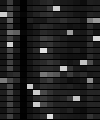
\includegraphics[width=7cm]{./imgs/br_model_all.png}};
		\matrix [
			matrix of nodes, nodes in empty cells,
			right=1cm of bars.north east, anchor=north west, tight,
			row sep={4.22mm,between origins}, column sep=1cm,
		] (rules) {
			 0\&      1\\   
			 1\&      0\\   
			 1\&     \\   
			\&        0\\   
			\&       \\   
			 1\&     \\   
			 1\&     \\   
			\&       \\   
			\&        0\\   
			 0\&      1\\   
			 1\&     \\   
			\&        0\\   
			\&       \\   
			\&        0\\   
			\&        0\\   
			\&        0\\   
			 1\&     \\   
			\&       \\   
			\&        1\\   
			\&        0\\   
		};
		\matrix [
			matrix of nodes, nodes in empty cells,
			left=1cm of bars.north west, anchor=north east, tight,
			row sep={4.22mm,between origins}, column sep=1cm,
		] (numbers) {
			1\\2\\3\\4\\5\\6\\7\\8\\9\\10\\11\\12\\13\\14\\15\\16\\17\\18\\19\\20\\
		};
		\matrix [above=0.4cm of rules, matrix of nodes] {
			\texttt{full} \& \texttt{empty} \\
			1-rule \& 1-rule \\
		};
		\node [above=0.7cm of bars] {expected input per unit};
		\node [above=0.7cm of numbers] {encoding units};
	\end{tikzpicture}
	\caption{Visualization of the trained encoder and Boolean functions. Details
	are explained in the main text.}
	\label{fig:breakout-model-all}
\end{figure}
The large image in Figure~\ref{fig:breakout-model-all} contains 20 ``rows''.
The $i$-th row in this image is the \emph{expected input} region that the DBN
predicts, given an encoding vector of zeros except for a 1 at the $i$-th
position (we can do this backpropagation because the encoder is a
probabilistic model). It emerges an interesting result: the presence of each
brick is associated to at least one encoding unit. For example, when the
left-most brick is present, the third unit of the encoder is~1. The most
probable input is also affected by a prior probability. In fact, the fourth
brick, which is almost always down, is the same that the agent has learnt to
hit first. However, a strong prior probability doesn't mean that that brick
has no unit associated.

On the right of this image we see two columns of 0s and 1s \dots.

% TODO: binary: no need to look at interactions and other stuff. 

\subsection{Comments}

% TODO: semplice per RL ma non necessariamente per feature extraction. Dipende
% dalla complessità dei fluenti
% TODO: osservazioni semplici poco rumorose, MA non uniformemente distribuite
% TODO: seleziono uno di 2^n configurazioni. Non potevo farlo con un simbolo
% solo e non potevo con altre configurazioni intermedie senza legarlo ad altri
% simboli.
% TODO: sembrava banale ma non lo è: natura combinatoria
% TODO: raggiunto perfettamente

% Back to brak into sections
\let\sectionbreak\savedsectionbreak

\section{Montezuma's Revenge}
\subsection{Definitions}
\subsection{Training}
\subsection{Comments}

% TODO: crossover and mutation p
